\documentclass[letterpaper,twocolumn]{article}

\usepackage[top=0.5in, bottom=1in, left=1in, right=1in]{geometry}
\usepackage{float}
\usepackage{graphicx}
\usepackage{caption}
\usepackage{subcaption}
\usepackage{amsmath}
\usepackage{titlesec}

\titleformat{\section}[runin]
{\normalfont\normalsize\bfseries}{\thesubsection}{1em}{}

\title{Roll and Pitch Motion Control for Legged Locomotion on the Water Surface}

\author{\small Nitish Thatte, Mahdi Khoramshahi, Metin Sitti \\
        \small Carnegie Mellon University \\
        \small \{nitisht, khoram\} at andrew.cmu.edu, metin at cmu.edu
}
\date{}
\begin{document}

\maketitle

\section*{Motivation}
The Basilisk Lizard's striking ability to sustain highly dynamic legged locomotion on a range of surfaces from hard-ground to water is a remarkable feat \cite{glasheen1996hydrodynamic}. Most legged robots would have difficulty emulating this animal's ability to robustly locomote on yielding or deforming surfaces. Therefore, to explore the dynamics of legged locomotion in this regime, we are studying the design of a bio-inspired water-running robot. Analyzing water-running dynamics may also help us gain insight into mobility on other yielding surfaces, such as granular media and mud. It is crucial that we develop locomotion models for these surfaces as robots continue to venture out of the laboratory and into the real world.


\section*{State of the Art}
The mechanical design of the water-running robot has undergone several design iterations. The current design, which can be seen in figure~\ref{fig:robot}, features four four-bar linkage legs producing  foot trajectories, as in figure \ref{fig:traj}, optimized for power consumption and lift. Park et al analyzed the roll and pitch dynamics of this robot and proposed an active tail for achieving stable robot pitch angles \cite{park2010roll}. However, addition of an active tail requires integration of another actuator, adding mass and complexity. Furthermore, no method for controlling roll angles has been proposed as of yet.




<<<<<<< HEAD
\section*{Own Approach}
To control the roll and pitch motion of the robot we propose a novel, closed-loop CPG that modulates the velocity of each foot during the downwards and upwards phases of their trajectories (Duty Factor), while simultaneously maintaining the phase relation between feet to perform trot gait. This approach takes advantage of non-linear fluid drag forces to generate differing forces on each foot, thereby imparting moments on the robot. 
	
We start with designing height controller for simplified one-leg water-hopper. To deal with the hybrid and time-variant nature of the system we utilize a time averaging approach. We then approximate the generated force by foot trajectory as an linear expression with respect to duty factor. Finally we design our controller output (duty factor) to achieve a desired virtual model, here a spring with adjustable stiffness. In order to take care of unmodeled dynamics and uncertainties, A PID-controller is also added to outer control loop.\\
=======
\section{Own Approach}
To control the roll and pitch motion of the robot, we propose a novel, closed-loop central pattern generator (CPG) that modulates the velocity of each foot during the downwards and upwards phases of their trajectories using a control input parameter we call duty-factor. This approach takes advantage of non-linear fluid drag to generate differing forces on each foot, thereby imparting moments on the robot. 
	
To deal with the hybrid and time-variant nature of the system we utilize a time averaging approach. We then find the force generated by an approximated foot trajectory in order to yield an expression, which is linear in duty-factor, for the average lift force over a cycle.  Finally, we design a controller, based on this force equation, to achieve a desired spring-like virtual model.


\begin{figure}[tb]
	\centering
	\begin{subfigure}[c]{0.24\textwidth}
		\centering
		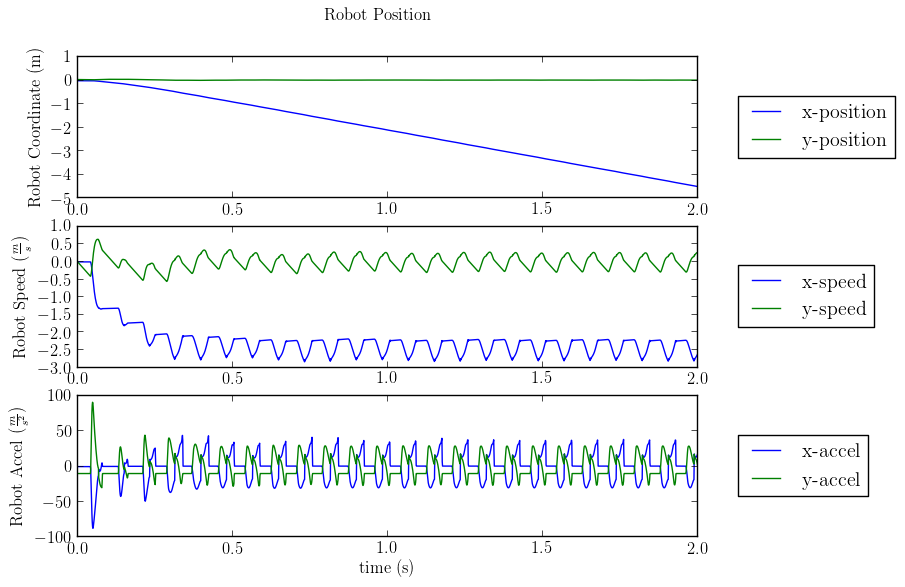
\includegraphics[width = \textwidth]{figures/robot.png}
	\end{subfigure}
	\begin{subfigure}[c]{0.24\textwidth}
		\centering
		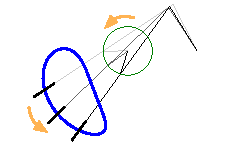
\includegraphics[width = \textwidth]{figures/traj.pdf}
	\end{subfigure}

	\begin{subfigure}[c]{0.24\textwidth}
		\caption{Robot Design}
		\label{fig:robot}
	\end{subfigure}
	\begin{subfigure}[c]{0.24\textwidth}
		\caption{Foot Trajectory}
		\label{fig:traj}
	\end{subfigure}
	\caption{}
\end{figure}
>>>>>>> 8d96567e3150335b9bd621f036a34b51884dd421

%Finally, we design a non-linear PID controller based on this force law, which attempts to minimize the error between the height of each corner of %the robot and a desired height, thereby achieving the desired roll and pitch angles.

\begin{equation}
	m \ddot{y} =  F(y,\dot{y},t,DF;A,\omega)
	\label{eq:force}
\end{equation}
\begin{equation}
	m \ddot{y} = F_{ave}(y,DF;A,\omega)
	\label{eq:force_ave}
\end{equation}
\begin{equation}
	m \ddot{y} = F_{s}(y,DF_0;A,\omega)D+F_{a}(y,DF_0;A,\omega)
	\label{eq:force_linear}
\end{equation}
\begin{equation}	
	D = F_{s}^{-1}(F_{vir}-F_{a})
	\label{eq:control}
\end{equation}
\begin{equation}	
	m\ddot{y} = F_{vir}
	\label{eq:virtual_model}
\end{equation}

\section*{Current Results}
In order to avoid fluctuations in controller because of oscillation (even though for fixed DF), we feed low-pass filtered height to the controller. Result of open-loop, Non-linear control, and NL-control with PID is illustrated in Fig??. Although the open-loop is stable, but DF should be set accordingly to desired height. NL control is able to reach the desired height, and it can be seen that PID can reduce settling time and steady state error. 

\section*{Best Possible Outcome}

\section*{Acknowledgment}
This material is based upon work supported by the National Science Foundation Graduate Research Fellowships. Any opinion, findings, and conclusions or recommendations expressed in this material are those of the authors(s) and do not necessarily reflect the views of the National Science Foundation.

\bibliographystyle{plain}
\bibliography{dynamic}

\end{document}
